\section{Skeletonization}

\noindent
\textbf{Volume Downsampling}
We downsample the segmentation data to a resolution of $30$ nm in each direction. 
The skeletonization algorithm that we use takes as a parameter the minimum distance between joints in the skeleton~\cite{zhao2014automatic}.
When we downsample, we also reduce this minimum distance by the same rate.
We find that this produces expressive skeletons at a fraction of the computational cost. 
Table~\ref{table:skeleton} shows statistics comparing the skeletonization algorithm on 200 randomly chosen labels.

\begin{table}
	\scriptsize
	\begin{center}
		\begin{tabular}{c c c c c} \hline
			& \textbf{Average Time} &  \textbf{Skeleton Length} & \textbf{No. Branches} & \textbf{No. Endpoints} \\ \hline
			Full Resolution & 16.35s & 1,352,157nm & 9,858 & 1,068 \\
			Downsampled & 0.56s & 1,671,138nm & 9,359  & 1,824 \\ \hline
		\end{tabular}
	\caption{The results of the skeletonization algorithm on both the full resolution and the downsampled data. Downsampling the data provides expressive skeletons at a fraction of the computational cost.}
	\label{table:skeleton}
	\end{center}
\end{table}

\begin{figure}
	\begin{center}
		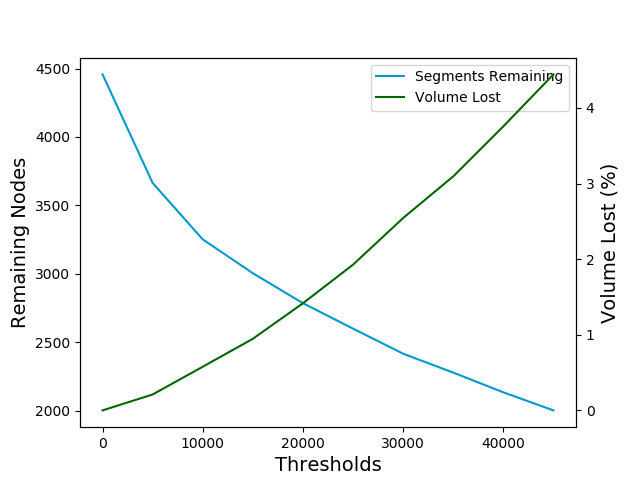
\includegraphics[width=0.45\linewidth]{./figures/node-threshold.png}
		\caption{The number of remaining nodes after increasing the threshold (blue) and the number of voxels excluded as a percent of the total volume (green).}
		\label{fig:node-pruning}
	\end{center}
\end{figure}

\noindent
\textbf{Node Generation}
We remove all nodes from the graph corresponding to labels with fewer than $t_{seg}$ voxels.
Figure \ref{fig:node-pruning} shows the results of varying $t_{seg}$ on two different quantities for the Kasthuri training volume. 
The blue line indicates the number of nodes remaining in the graph.
The rate of node reduction decreases for larger thresholds since there are fewer labels of larger size. 
The green line shows the percent of voxels with a label pruned from the graph.
Ideally this number is low since we want to remove small segments which do not contribute much to the overall volume.
This ``volume lost" grows at an increasing rate as the larger segments are removed. 
Based on these curves we set $t_{seg} = 20,000$ voxels.
With this threshold, we prune over half of the labels and only lose $1.5\%$ of the total volume.
